\begin{figure}[htbp]
\section*{ ROR2}
\centering
\begin{subfigure}[b]{0.95\textwidth}
\centering
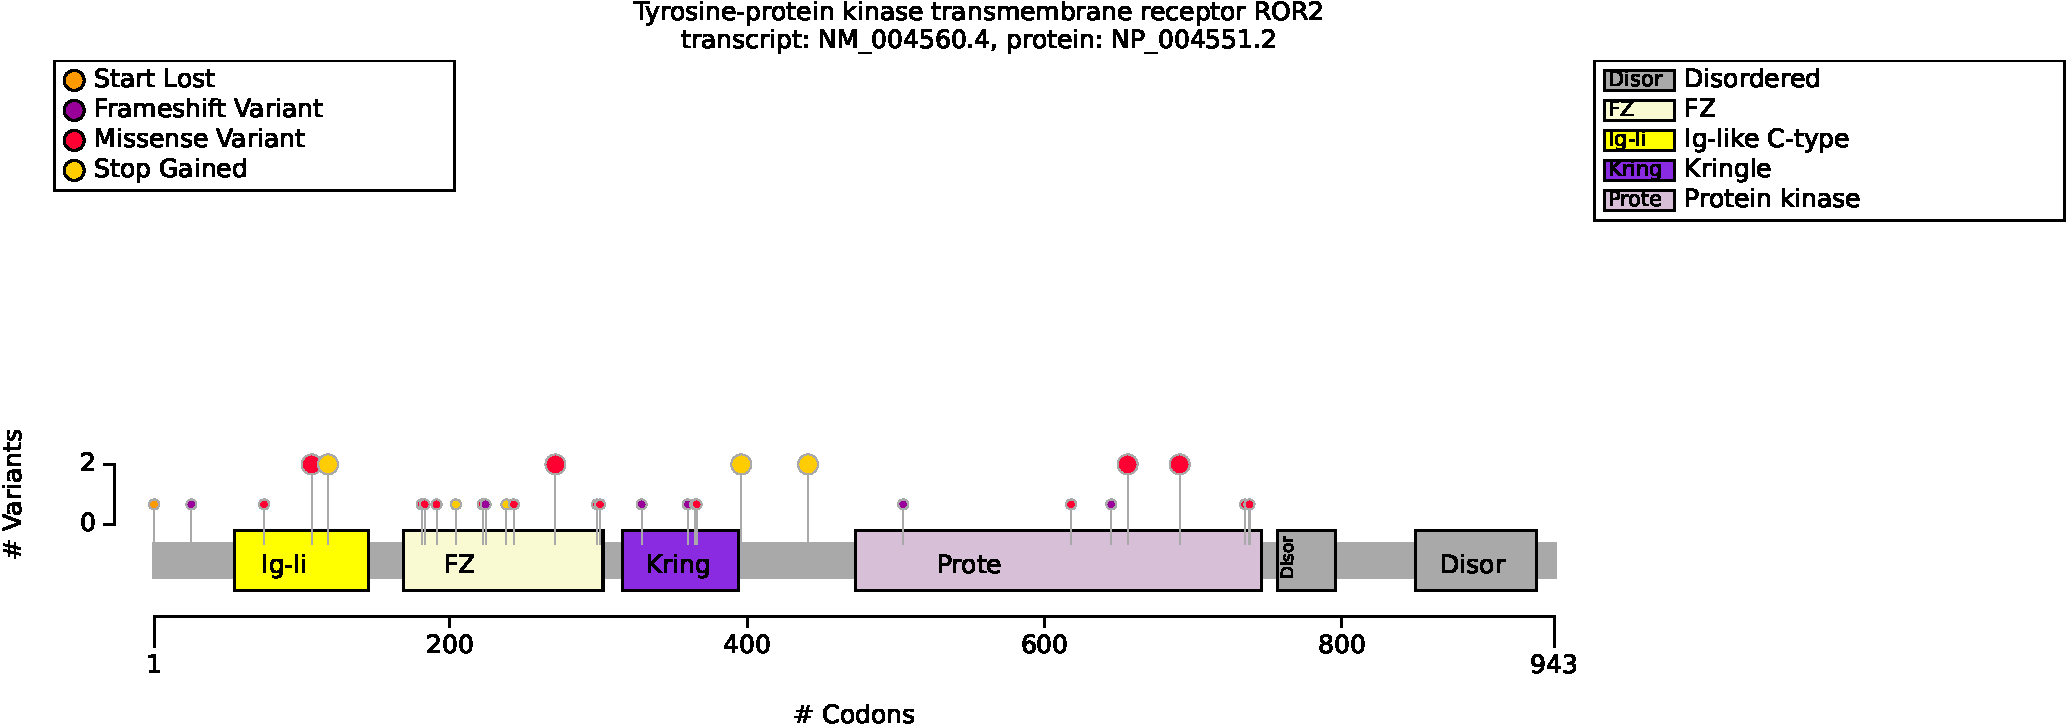
\includegraphics[width=\textwidth]{ img/ROR2_protein_diagram.pdf} 
\captionsetup{justification=raggedright,singlelinecheck=false}
\caption{Distribution of variants in ROR2}
\end{subfigure}

\vspace{2em}

\begin{subfigure}[b]{0.95\textwidth}
\centering
\resizebox{\textwidth}{!}{
\begin{tabular}{llllrr}
\toprule
Genotype (A) & Genotype (B) & total tests performed & significant results\\
\midrule
missense/missense OR missense/other & other/other & 116 & 0\\
FZ domain/FZ domain OR FZ domain/other & other/other & 116 & 0\\
\bottomrule
\end{tabular}
}
\captionsetup{justification=raggedright,singlelinecheck=false}
\caption{             Fisher Exact Test performed to compare HPO annotation frequency with respect to genotypes. }
\end{subfigure}

\vspace{2em}

\caption{ The cohort comprised 32 individuals (3 females, 7 males, 22 with unknown sex). A total of 81 HPO terms were used to annotate the cohort. Disease diagnosis: Robinow syndrome, autosomal recessive (OMIM:268310). No statistically significant genotype-phenotype correlation was identified. A total of 32 unique variant alleles were found in \textit{ROR2} (transcript: \texttt{NM\_004560.4}, protein id: \texttt{NP\_004551.2}).}
\end{figure}
